\section{Results}

	\subsection{ring networks}

\begin{figure}\label{fig:N8_uni_ring_dynamics_capacities}
	\centering
	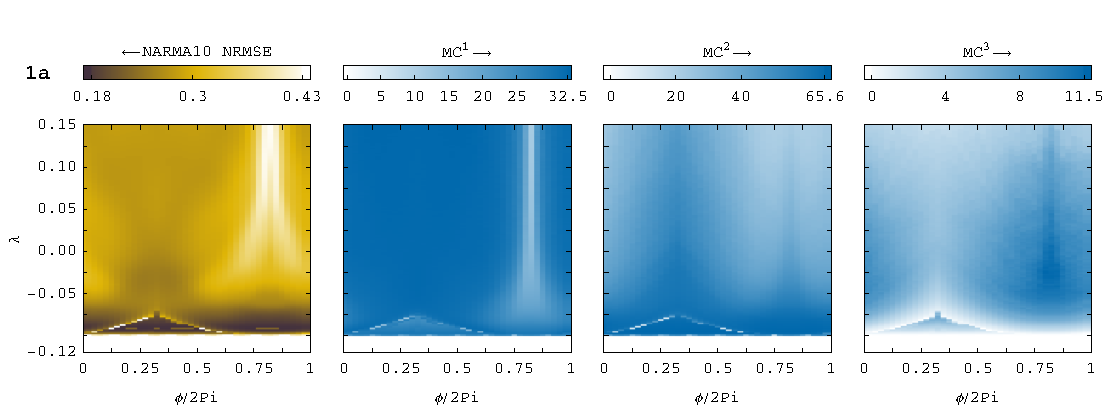
\includegraphics[width=15cm]{pics/N8/basics/N8_1a_uni_th3_tau68_vN16_capacities}
	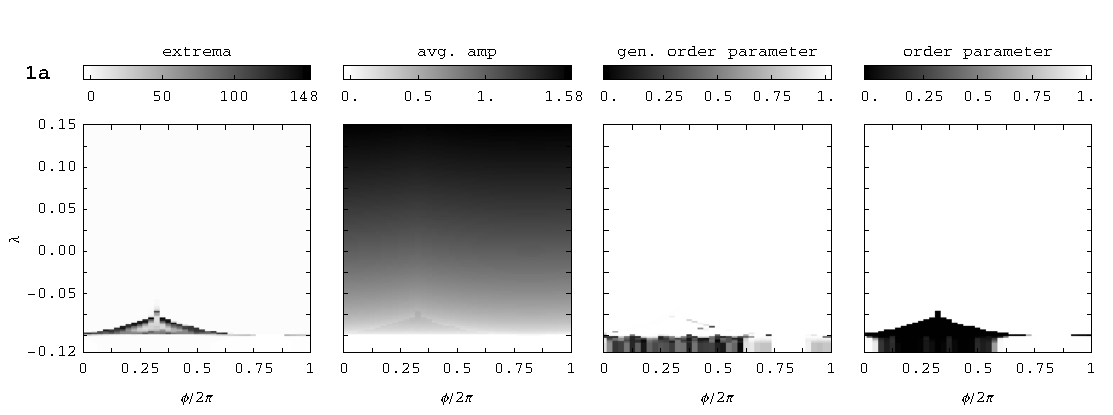
\includegraphics[width=15cm]{pics/N8/basics/N8_1a_uni_theta3_tau68_dyn}
	\caption{$N_r=8$: the unidirectional ring (network \textbf{1a} in Fig.:\ref{N8_uni_w_extra}). NARMA10 error, memory capacities $MC^{d}$ and dynamical indicators are shown over $\lambda$ and coupling phase $\phi$ with $\tau=68$ $\theta=3$ $\kappa=0.1$. Arrows indicate greater performance.}
\end{figure}


\begin{figure}\label{fig:N8_basics_ring_capacities}
	\centering
	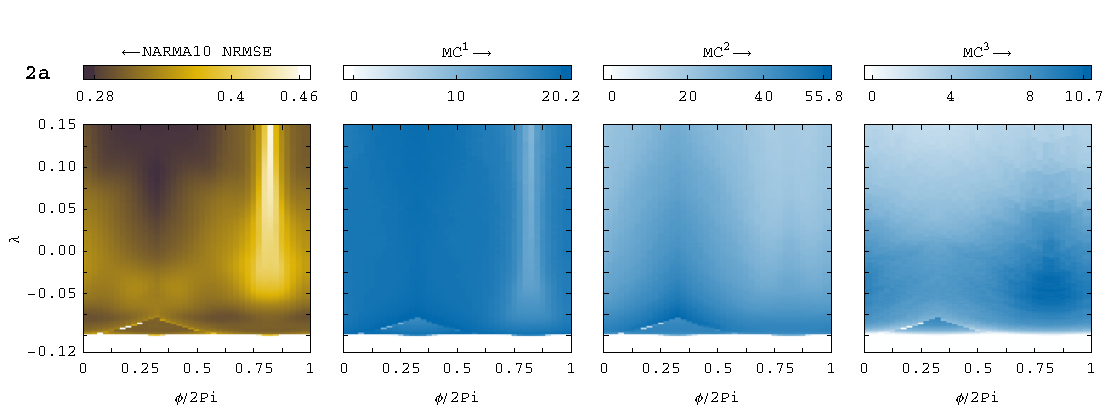
\includegraphics[width=15cm]{pics/N8/basics/N8_2a_bidir_th3_tau68_vN16_capacities}
	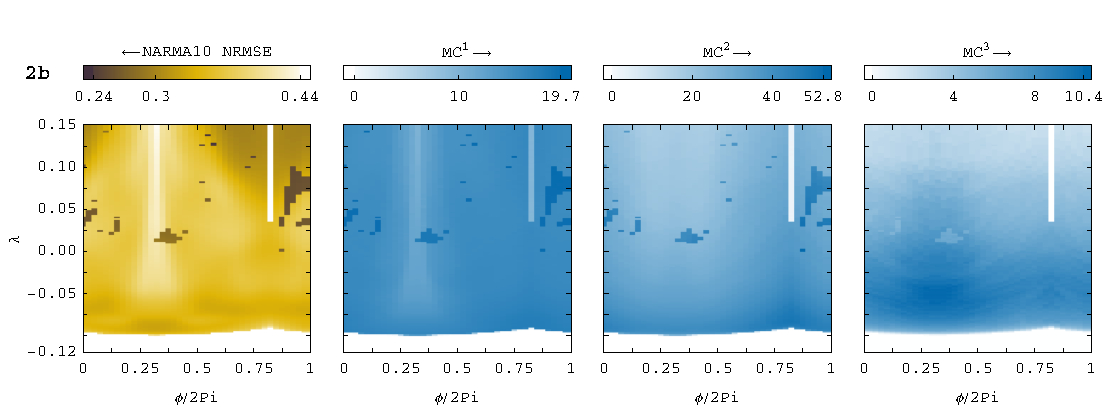
\includegraphics[width=15cm]{pics/N8/basics/N8_2b_diffuse_th3_tau68_vN16_capacities}
	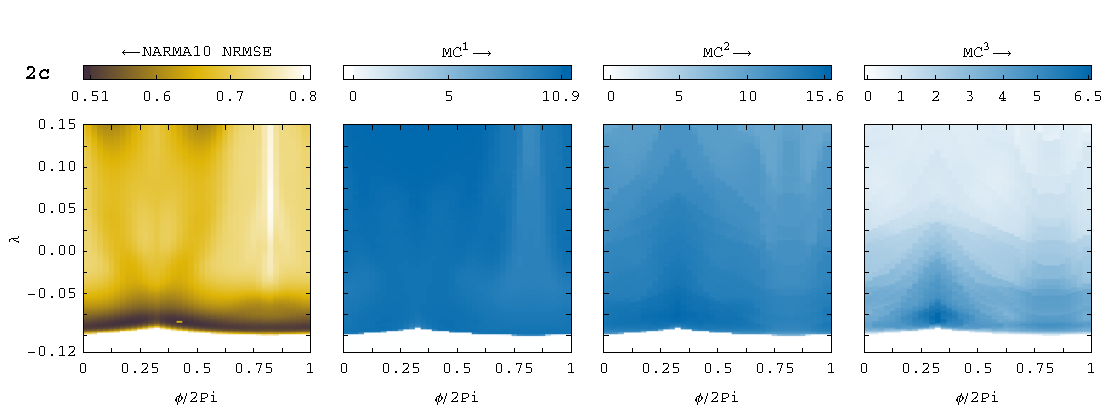
\includegraphics[width=15cm]{pics/N8/basics/N8_2c_all2all_th3_tau68_vN16_capacities}		
	\caption{$N=8$: several highly symmetric (ring-)topologies: bidirectional ring \textbf{2a}, diffuse-coupled ring \textbf{2b} and the complete graph \textbf{2c}.
		Other parameters: $\tau=68$ $\theta=3$ $\kappa_i=0.1$)}
\end{figure}
		
		\begin{figure}\label{fig:n8_uni_ring_tau_cc_capacities_syncandsplay}
			\centering
			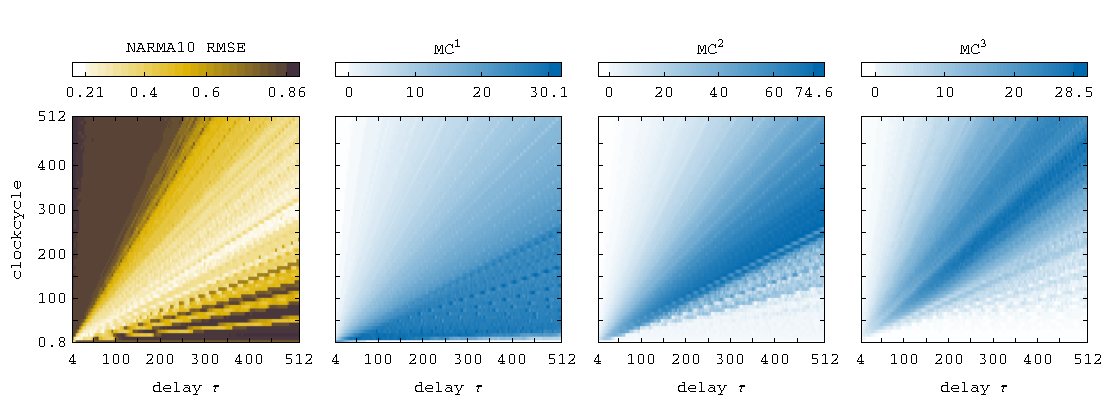
\includegraphics[width=15cm]{pics/n8_narmaplot_sync}
			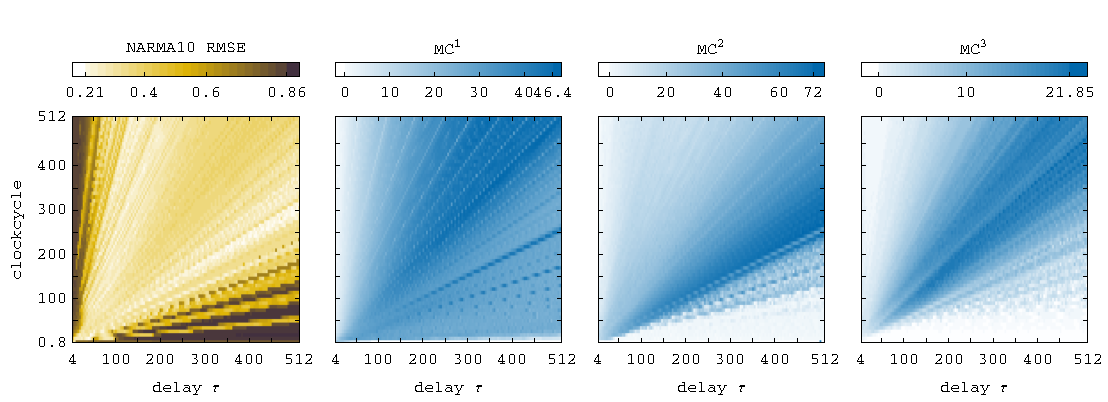
\includegraphics[width=15cm]{pics/n8_narmaplot_splay}
			\caption{Several capacities in a unidirectional ring network $N=8$ with $N_v=16$. Shown are capacities over delay $\tau$ and clockcycle $T$ for \emph{synchronized state} (top) and \emph{splay state} (bottom). Depending on the state the capacities are different.}	
			\label{fig:n8_uni_ring_tau_cc_capacities_syncstate}

		\end{figure}

	\subsection{Highly symmetrical network topologies}

			\begin{itemize}
				\item unidirectional ring
				\item bidirectional ring
				\item diffuse coupling (bidirectional coupling with equalizing self-links)
				\item all-to-all coupling including self-links
			\end{itemize}

				
	
		
		Rings with from N=1(edge case) to N=16
		Bidirectional Rings
		Bidirectional Rings with self-feedback and diffuse coupling
		
		\subsection{All to all coupled networks}
		N=3 - N=16 row normalization
		
	\subsection{Less symmetrical network topologies}
		\subsubsection{unidirectional rings with jumps}
			
		
